\chapter{Popis navrženého řešení a použitých technologií}

\section{OpenStack}\label{sub:interaction}

Popis Openstacku

\subsection{Heat Templates}

Popis co jsou to heat templates.

Heat is the main project of the OpenStack orchestration program. It allows users to describe deployments of complex cloud applications in text files called templates. These templates are then parsed and executed by the Heat engine.

\begin{figure}[h]
\begin{centering}
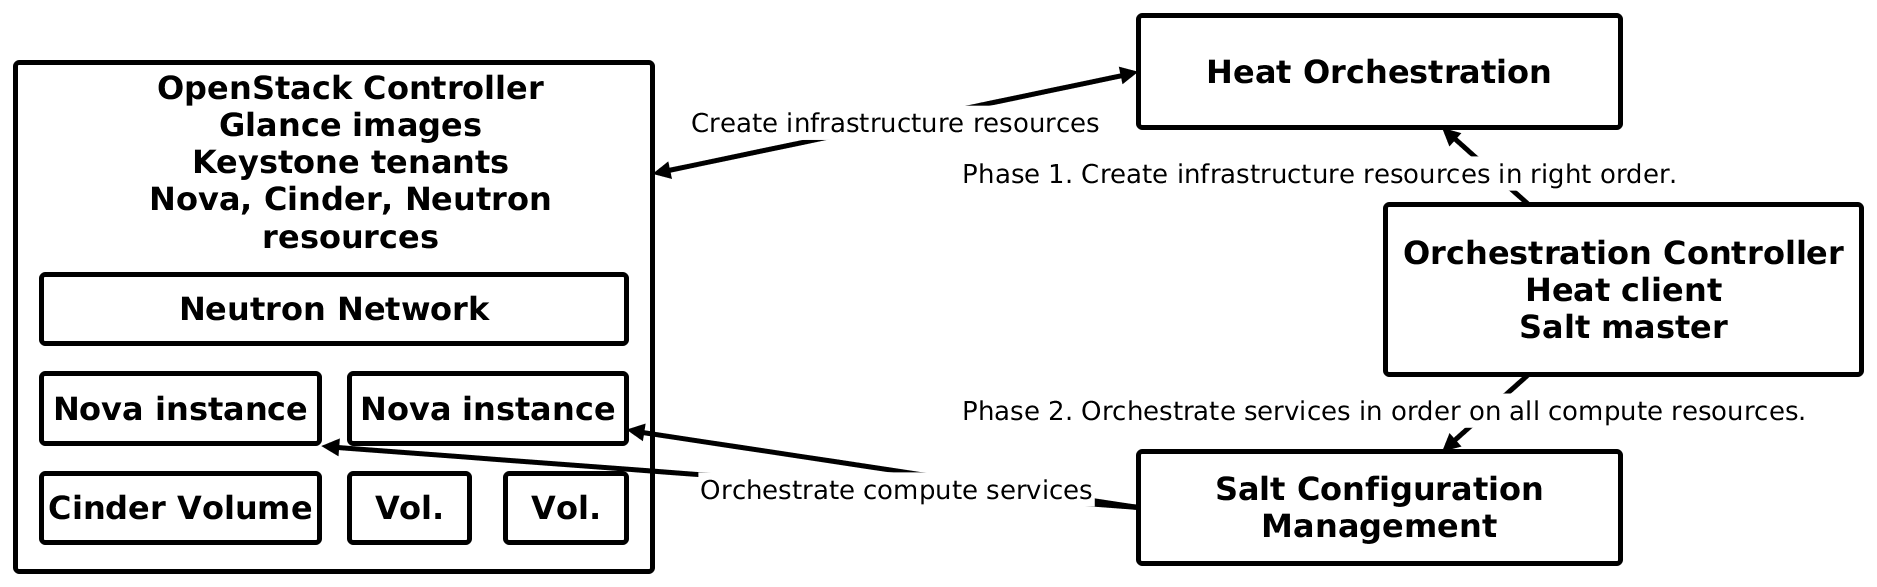
\includegraphics[scale=0.21]{images/heat}
\par\end{centering}
\caption{Popis heat orchestrace\label{fig:heat}}
\end{figure}

OpenStack Heat Templates are used to demonstrate load balancing and firewalling inside of Openstack.

\section{OpenContrail}\label{sub:interaction}

Popis OpenContrailu.

\subsection{Service Chaining}

Popis service chaining v contrail a service instanci.
a jak to může být využito pro VNF.